\documentclass[10pt,a4paper]{article}
\usepackage[english]{babel}
\usepackage{amsmath}
\usepackage{amsfonts}
\usepackage{graphics}
\usepackage{epsfig}
\usepackage{amssymb}
\usepackage{graphicx}
\author{Elisabeth Lindquist, Fredrik Lundell, Johan Peterson}
\title{\textsc{Deformation of tetrahedral meshes using the Finite Element Method}\\\begin{small}\textsc{Tsbk03 - Advanced game programming}\end{small}}
\begin{document}
\maketitle
\begin{abstract}

\end{abstract}
\pagebreak
\tableofcontents
\pagebreak

\section{Introduction}
In the real world all materials are deformable in some extent. Even something
as solid as a diamond can be deformed using the right amount of force. How to
represent the physical properties of an object varies upon the application. It is
common to use a rigid body model for simulating a solid object although other
methods is needed to capture the inner dynamics of an object.
The finite element method has a long history and where mainly originated
from the need of solving complex structural analysis problems in civil engineering.
It has successfully been used for stress analysis and this approach is
applicable for simulating how a object deformers during stress.
There is however simpler methods for simulating deformable objects for
example a mass-spring system. A mass-spring system defines the object as a
set of particles interconnected by springs. The behavior of the system depends
on how each spring is connected and the number of springs holding the object
together. The implementation is kind of straight-forward although [1] points
out some drawbacks using this method for deforming 3D object.

Real time physics: \cite{rt_phys}.
\section{Method}

\subsection{Physical body Mechanics}
The elasticity of a material is often expressed with Hook's law approximated as a linear combination of stress and strain\ref{ett}.

\begin{equation}\label{ett}
    \frac{F_{n}}{A} = E \frac{\triangle l}{l}
\end{equation}
External forces acting on a surface gets transmitted through the material causing inner forces a quantity described as stress. This stress acting on a body gives rise to strain an measurement of deformation defined as the relatively elongation or compression of the material.

In one dimension the stress $\sigma$ is a scalar describing the force $ F_{n}$ acting perpendicular to the surface cross-sectional area $A$.
This force causes deformation or strain defined as the difference in length of the material perpendicular to the surface $\triangle A$. Stress and strain is related through Young's modulus $E$ which states the stiffness of the material.

\subsubsection{Stress and Strain in three dimensions}
In three dimensions the stress and strain is different depending on the direction of measurement. A point can be strained in one direction and compressed in another thus stress and strain cant be expressed with a single scalar.

A displacement field $\mathbf{u}$ is described as the difference of each points in its initial and deformable state. Hence a point can be strained differently in all direction $\mathbf{u}$ is a vector field described in \ref{tva}.


\begin{eqnarray}\label{tva}
    \mathbf{u}(x, y, z) = \left[ \begin{array}{c}
u(x, y, z) \\
v(x, y, z) \\
w(x, y, z) \end{array} \right]
\end{eqnarray}

The point $x$ new position can be evaluated through the displacement field $p=x+\mathbf{u(x)}$
where $p+dp = x+dx + \mathbf{u(x+dx)} => dp = dx + \mathbf{u(x+dx)}-\mathbf{u(x)} = dx +\nabla \mathbf{u(x)}dx$. Where $\nabla \mathbf{u(x)}$ is the gradient of the displacement field $u$. The strain tensor is a 3x3 matrix and can be derived from the spatial derivatives of the displacement field as illustrated in equation \ref{tre}

\begin{equation}\label{tre}
    \epsilon = \bigtriangledown u + \bigtriangledown u^{T} + \bigtriangledown u^{T} \bigtriangledown u
\end{equation}

This tensor is called Green’s strain tensor and is symmetric and nonlinear. The tensor has the important property of behaving linear for small deformations
and by removing the nonlinear term, Cauchy’s strain tensor is formed. The tensor is illustrated in equation 4 where $\epsilon_{xx}, \epsilon_{yy}, \epsilon_{zz}$ is represents normal strain and $\epsilon_{xy}, \epsilon_{xy}, \epsilon_{xz}$  shear strain.

\begin{eqnarray}\
\epsilon =  \left[ \begin{array}{cccc}
\epsilon_{xx} & \epsilon_{xy} & \epsilon_{xz} \\
\epsilon_{xy} & \epsilon_{yy} & \epsilon_{yz} \\
\epsilon_{xz} & \epsilon_{yz} & \epsilon_{zz} \\
 \end{array} \right]
\end{eqnarray}

In coherency with strain, three dimensional stress also varies in the direction of measurement. As a result, stress is represented as a 3x3 tensor as shown in equation \ref{fem}.

\begin{eqnarray}\label{fem}
\sigma =  \left[ \begin{array}{cccc}
\sigma_{xx} & \sigma_{xy} & \sigma_{xz} \\
\sigma_{xy} & \sigma_{yy} & \sigma_{yz} \\
\sigma_{xz} & \sigma_{yz} & \sigma_{zz} \\
 \end{array} \right]
\end{eqnarray}
Where $\sigma \cdot n = \frac{dF_{n}}{dA}$ gives the stress measuring in direction $n$.

\subsubsection{Redefine Hook's Law}
Assuming an linear relationship between stress and strain Hooke's law can be redefined as equation \ref{sex}.

\begin{equation}\label{sex}
    \sigma = E \cdot \epsilon
\end{equation}

 $E$ is the connection between stress and strain and depends on properties of the material. For simplicity only isotropic materials is considered, isotropic meaning that the material properties are independent of directions. Material such as plastics or different kinds of alloys are examples of isotropic materials where wood is an example of an anisotropic material which is weaker along rather than across the grains.

Both stress and strain is represented with symmetrical 3x3 tensors. Symmetrical 3x3 matrices only depend on 6 variables hence
$\sigma$ and $\epsilon$ is vectors of dimensionality 6x1. $E$ can then be defined as 6x6 matrix which for isotropic materials only depends on two elastic constants, Young's modulus $E$ and the Poisson's ratio $\nu$. Young's modulus is the ratio of stress or elasticity and Poisson's ratio describes to which amount volume is conserved. Using these notations Hook's law now can be written as equation \ref{sju} assuming the use of isotropic materials.

\begin{eqnarray}\label{eqn:ststhooks}
\left[ \begin{array}{c}
\epsilon_{xx} \\
\epsilon_{xx} \\
\epsilon_{xx} \\
\epsilon_{xx} \\
\epsilon_{xx} \\
\epsilon_{xx} \\
\end{array} \right] = \frac{E}{(1+\nu)(1-2\nu)}
\left[ \begin{array}{cccccc}
1-\nu & \nu & \nu & 0 & 0 & 0\\
\nu & 1-\nu & \nu & 0 & 0 & 0\\
\nu & \nu & 1-\nu & 0 & 0 & 0\\
0 & 0 & 0 & 1-2\nu & 0 & 0\\
0 & 0 & 0 & 0 & 1-2\nu & 0\\
0 & 0 & 0 & 0 & 0 & 1-2\nu\\
 \end{array} \right]
\left[ \begin{array}{c}
\epsilon_{xx} \\
\epsilon_{xx} \\
\epsilon_{xx} \\
\epsilon_{xx} \\
\epsilon_{xx} \\
\epsilon_{xx} \\
\end{array} \right]
\end{eqnarray}



\subsection{Discretization using Finite element method}
The finite element method (FEM) is a well known numerical method for approximating a solution to a continues problem. The whole domain is sampled into a set of finite elements and as elements volume converges to zero FEM becomes an highly accurate approach for approximating a analytical solution. FEM has been around for decades and is applicable to a wide range of physical and engineering problems such as mechanical, structural and thermal analysis.

\subsubsection{Local stiffness of a tetrahedron element}
The volume of the deformable object is divided into a finite number of linear tetrahedral elements. A tetrahedron is an three dimensional object which has four nodes each having three degrees of freedom.

\begin{figure}[h]
\centering
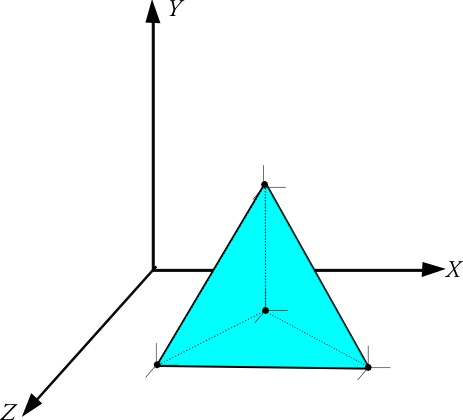
\includegraphics[width=.3\columnwidth]{figures/tetra_coord.png}
\caption{}
\label{fig:4}
\end{figure}

The displacement field $u(x,y,z)$ is continues and must be discretisized in order to use the finite element approach. In equation \ref{nio} the displacement field $u(x,y,z)$ is obtained by using $N(x,y,z)$ which is a 12x3 matrix containing the shape functions used to interpolate displacement values inside the tetrahedron. The shape matrix is multiplied with the displacement vector $\hat{u}$ as in \ref{nio}, $\hat{u}$ is a 12x1 vector containing the displacement x,y,z at each node of the tetrahedron. This multiplication gives a approximated displacement field $u(x,y,z)$ which is constant for the whole tetrahedron.

\begin{equation}\label{nio}
    \mathbf{u} \approx N(x,y,z) \hat{u}
\end{equation}

To obtain the strain tensor $\epsilon$ the approximated displacement field is multiplied by L which essential consist of differential operators used to get the partial differential of $u$.

\begin{equation}\label{tio}
    \epsilon = LN \hat{u} = B_ {e} \hat{u}
\end{equation}

$B_ {e}$ is called the strain matrix which is constant and can be precomputed for all elements.

As a result of the strain matrix $B_{e}$ the entire stiffness of the tetrahedron element can be expressed as the stiffness matrix $K_{e}$ connecting all degrees of freedom of a tetrahedron. The element stiffness matrix is calculated in equation \ref{eqn:stiffnessmatrix} where $V_{e}$ is the volume of the element and $E$ is the material properties defined in \ref{eqn:ststhooks}.

\begin{equation}\label{eqn:stiffnessmatrix}
    K_{e} = V_{e} B_ {e}^{T}EB_ {e}^{T}
\end{equation}

The element stiffness matrix describes the relationship between all degrees of freedom of a tetrahedron an relates through Hook's law as equation  

\begin{equation}\label{eqn:stiffnessmatrix}
    f_{e} = K_ {e}\hat{u}
\end{equation}

If a node displacement occurs this relationship gives the interconnecting forces accumulated for all node spanning the finite element.

\subsubsection{Global stiffness of a tetrahedron mesh}
For the purpose of a global solution all local stiffness matrices $K_{e}$ is assembled into global stiffness matrix $K$. The assembling process is not trivial and need to be composed in way so that a force affecting one elements deflect the others through the body. How to compose the global stiffness matrix from different types of finite elements etc.

 Since a large part of the dynamics in the global stiffness matrix $K$ is overlapping $K$ tends to be sparse. The dimensionality of $K$ is $3 \cdot n x 3 \cdot n$ where 3 is the degrees of freedom and n is the number of nodes inside the entire object.
 
\subsection{}
\subsection{}


\section{Implementation}


\subsection{Tetrahedron mesh}
When using the FEM in a volume application, such as ours, a mesh of tetrahedral objects is used. This mesh need to be generated and stored in a suitable data structure.

\subsubsection{Volume generation}
The finite volume elements can be generated in several ways. To create a tetrahedral mesh from a triangle mesh different triangulation methods can be applied. Snice this problem is not the main focus of the project already created tetrahedral objects are used. These are defined as two lists, one containing all vertex points in the tetrahedrons and one containing a list of which vertices that belong to each tetrahedron.

The vertex positions are read from the file and temporarily stored. For each tetrahedron in the tetrahedron list the corresponding vertex indices are found, the positions read and a tetrahedron object is created using these position. The vertices must be placed in an order that results in a tetrahedron with a positive volume. The function for creating a tetrahedron calculates the volume and if it is negative it makes a recursive call with the vertices in a different order.

We have defined the positions and vertex indices of a cube consisting of five tetrahedrons, and also tested our application using some of the meshes created by M\"uller-Fischer \cite{meshes}.


\subsubsection{Data structure}
In order to access the data in efficient way it must be stored in a suitable data structure. We have implemented a data structure consisting of the classes \texttt{Vertex}, \texttt{Face}, \texttt{HalfEdge}, \texttt{Tetrahed} and \texttt{TetrahedMesh}. This structure was inspired by the Compact Half-Face data structure introduced by Lage et al. \cite{halfface}, which has features that makes it possible to optimize for things such as execution speed and memory consumption. We have, however, decided to implement only the parts of the data structure that we have found to be necessary for our application. We have also made some simplifications and changes, where we have favored ease of use with our methods over speed and memory consumption.

\subsubsection{Primitives}
The primitives of a tetrahedral mesh are used to store vertex positions and keeping track of information such as adjacency and face normals. The \texttt{Vertex} class contains functions for setting and retrieving vertex positions. A \texttt{Vertex} also belongs to a \texttt{HalfEdge}, and the corresponding \texttt{HalfEdge} is stored for each \texttt{Vertex}. The \texttt{HalfEdge} class contains functionality for traversing the data structure by keeping the indices of its \texttt{next}, \texttt{prev} and \texttt{pair} \texttt{HalfEdge}. Its functionality is similar to the Half Edge data structure for triangular meshes described by Botsch et al. \cite{Botsch}. Each \texttt{HalfEdge} has a \texttt{Face} related to it, and keeps the corresponding index. The \texttt{Face} class also keeps track of which \texttt{Face} belong to which \texttt{HalfEdge}. A \texttt{Face} also has a normal, that can be set and retrieved. It also keeps the indices of its opposite \texttt{Face}. A tetrahedron is represented by the \texttt{Tetrahed} class, which keeps the indices of a \texttt{Vertex}, a \texttt{HalfEdge} and four \texttt{Faces}.


\begin{figure}[htbp]
\label{fig:tetraedge}
\begin{center}
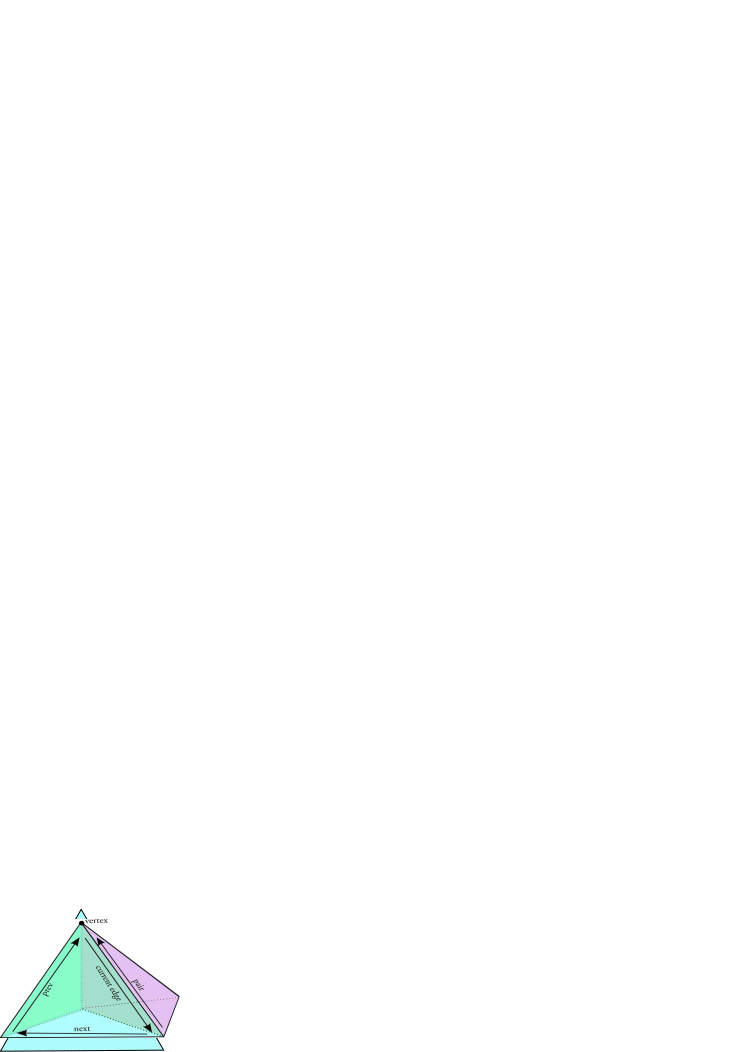
\includegraphics[scale=1]{figures/tetra_edge}
\caption{The Half Edges of a face.}
\end{center}
\end{figure}

\begin{figure}[htbp]
\label{fig:tetraface}
\begin{center}
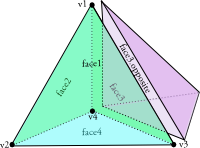
\includegraphics[scale=1]{figures/tetra_face}
\caption{The faces of a tetrahedron.}
\end{center}
\end{figure}


\subsubsection{The \texttt{TetrahedMesh} class}
The \texttt{TetrahedMesh} class contains functions for creating, changing and rendering a tetrahedral mesh.

\subsection{The \texttt{Solver} class}
\subsubsection{}
\subsubsection{}
\subsubsection{}
\subsection{Conjugate gradient solver}

\subsection{Graphical user interface}

\subsection{Rendering the result}


\section{Results}
\subsection{Images}

\subsection{Performance}

\section{Discussion}
\subsection{Improvements and further work}
\subsubsection{Solution on the GPU}


\subsubsection{Collision detection}


\pagebreak
\addcontentsline{toc}{section}{References}
\bibliographystyle{vancouver}
\bibliography{refs}
\end{document} 